\documentclass[a4full,12pt]{article}

\title{Integrating a Category-Partition Testing Tool with Combinatorial Interaction
Testing Tool To Produce T-Way Adequate Test Frames}
\author{Andrew Graff}

%\usepackage{fullpage}
%\usepackage{epsfig}
\usepackage{graphicx}
\usepackage{xcolor}
\graphicspath{ {./images/} }

\newcommand{\eas}[1]{{\color{blue}\sf ({#1})}}

\begin{document}
\maketitle
\section{Introduction}
\eas{Start with stating that software has defects and those defects can be costly. That is, first you need to make a point why it is important to have defect/bug free software.} Testing is an important step in the process of creating useful \eas{may be defect-free?} software. Who is
  going to use or buy your product if it doesn't function according to the  specifications?\eas{Let's focus on defects/bugs and not on the specification. You can rephrase this sentence in terms of testing and move it up so it is before ``Testing is an important ...''}.  For this reason, there are countless hours dedicated to  testing, debugging and maintaining software so that it performs the work expected of it.\eas{Once again, let's focus on testing. You can state that testing is a difficult problem and there may approaches for testing: black-box, white-box} It can be a challenge to create a sustainable, thorough, and comprehensive test suite that is efficient and effective at testing software.\eas{This statement is too general. Instead it should bring up the problem you are trying to address. You can say that various testing technique are complementary in their approaches and it would be beneficial to combine/integrate those components together. }
  
  
\section{Project Statement\eas{Problem Statement and Proposed Solution}}
  \eas{Here you can state the main point of what you are proposing -- combining TSL (testing specification language), i.e., the front-end of the category partitioning method with combinatorial interaction testing, which has no useful front-end}
  
Category partitioning is a useful \eas{blackbox testing} approach  \eas{that helps testers systematic design test case}. In particular it breaks up\eas{partitions, divides} a software system\eas{ or its inputs? into categories} to be tested, and when combined with TSL, can be useful for generating all possible test cases for the given system partition. \eas{you need to have at least 5 more sentences here mainly stating advantages of the category partition level, that TSL is the front-end and allows users to clearly express the input partitions. At the same time you need to tell the main draw-back of this approach -- it generates all test cases, which can be too many even with additional ``coarsening'' of the categories and their choices}

\eas{Here you can start that combinatorial interaction testing addresses this problem by finding test cases where only certain category choices appear together}
 Similarly, combinatorial interaction testing is useful for defining a subset of tests that satisfy a t-way pairwise interaction using a model and constraints file. \eas{Give three to four more sentence about how  CASA tool does it}\eas{ Then talk about its front end -- in fact its front-end is quite confusing that might introduce errors especially when expressing constraints. You might also state that in general an industry tester would not be able to use such tool --- how many would be able to express a constraint in a conjunctive normal form? Or decode the resulting output file.}
 
\eas{Here you should talk how you propose to solve this problem. The goal of this project is to ...} These two methodologies and tools\eas{you never mentioned any tools -- mention them in their corresponding paragraphs} are separate pieces of software that require the user  to generate the input to both tools. This project takes on the task of combining\eas{the user-friendly input/output components of one and integrate them into powerful test selection algorithm of another} these two powerful methods and tools so that the user only needs to generate the category partition test specification, and an adequate coverage set of test frames is generated eliminating the need for the engineer to create the model or constraints for the combinatorial interaction testing.

  
\section{Background}
\eas{Have  a better transition, e.g., This section presents background information on both methodologies and their corresponding tools. In particular, ...}
This project builds on the work of two teams that have come up with solutions to
  two different problems. Here we will explain each of those solutions and the 
  tools created to support them.

The \emph{category-partition method} uses a formal test specification language to generate
  test case descriptions. These test case descriptions would then be used to
  create an executable software test. So how do you generate the formal test 
  specifications? Depending on the size of the software system to test, the 
  engineer may need to break the program up into smaller testable blocks. For 
  the purposes of this project, we will use a simple example of a zip command.
  The test specification file can be seen in Fig. \ref{fig:tsl_input}.\eas{I have not given much of feedback here since it does need substantial information on
  \begin{itemize}
  \item The idea of black-box testing -- test selection based on the input space of a progra
  \item Partition of the input space into equivalent classes
  \item Category partition method as a systematic way multi-level way of partition the input space
  \item TSL as a formal language to express those categories and paritions
  \item Existence of constraints between choices of different categories
  \item Resulting frames
  \item Refinement and coarsening of the spcification
  \item The tool description - lines of code and such
  \end{itemize}
  Also the example on Figure~\ref{fig:tsl_input} is too large - try create something smaller, similar what we use in class -- new link in a browser setting
  }
\begin{figure}[-htb]
\centering
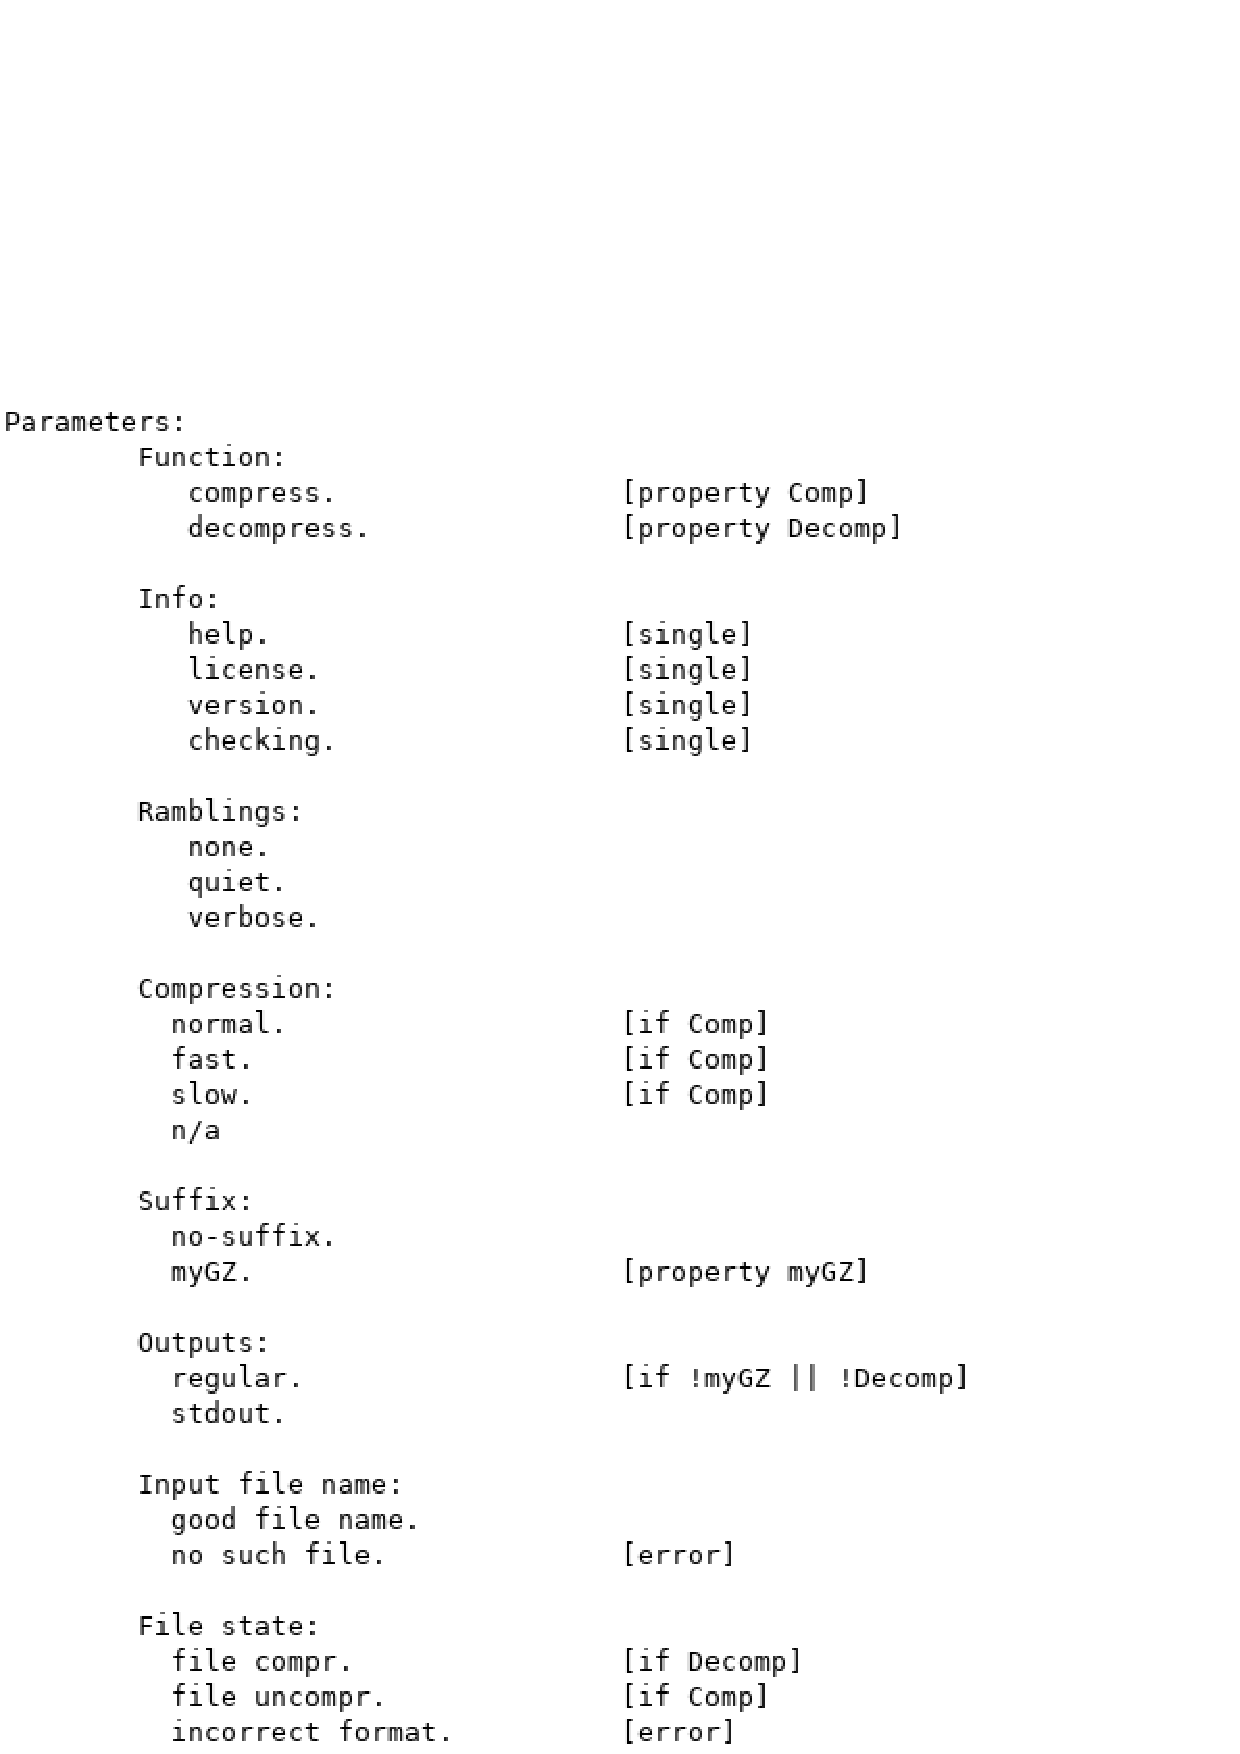
\includegraphics[width=3in,keepaspectratio]{tsl_input.png}
\caption{Category partition input format}
\label{fig:tsl_input}
\end{figure}



Combinatorial Interaction Testing -
\eas{Make sure you address the following
\begin{itemize}
\item The premise of t-way testing (defects occurs when few choices of categories interact, e.g., two choices)
\item An overall approach of CIT test case selection.
\item CASA tool and its input and output format examples, emphasize that it is not user-friendly. Moreover, a compound constraint among choices should be converted into a conjunctive normal form (CNF), i.e., "AND" of "ORs" between choices
\item Have some metric of this tool - lines of code and such
\end{itemize}
}

\section{Preliminary Work}
Some preliminary work has been done on this project in order to determine if
  the work is sufficient for submission\eas{to determine the feasibility of the approach}. One of the goals of the project is to
  combine\eas{be more specific - the front-end of one with the algorithm of another} the \emph{tsl} tool with the \emph{casa} tool. Source code was
  acquired for both tools and some initial study of the code was done. As it
  turns out, the \emph{tsl} tool is written in basic C. \emph{casa} on the other
  hand is written in C++. Converting \emph{tsl} to C++ would be beneficial if
  code is to be combined, so that tool has been updated to compile with the g++
  compiler.

  
Another goal of this project is to require the user to only generate the
  category partition test specifications, and the adequate coverage set of test
  frames should be generated.  Excluding the constraints file that would be used 
  by \emph{casa} to determine which options can be called with other options, a
  preliminary working version of \emph{tsl} was coded to output the 
  combinatorial interaction testing model required to generate a set the set of
  test frames that would be generated with no constraints.\eas{That is a long sentence, could you break it into tow or three?} 
  
    
  \eas{I think below you have all the information written well. However it would be better if instead of starting a paragraph talking about \em{what you've done} and then \em{why you did it}, you switch the order. State first what needs to be done: (1) establishing the map between categories and their choices and casa input values; (2) invoking casa on the translated input; (3) interpreting casa's output to produce frames}
  
  In order to achieve this, a new struct was added to \emph{tsl/structs.h} called \emph{container} that
  keeps track of the list of non-single Choices as a vector of Choice struct
  pointers.\eas{Make sure you explain in your background section what is Choice - by the way why is it capitalized?} This vector is used to lookup the choices and categories later for
  printing the test frames. In addition, a \emph{parent} pointer was added to
  the Choice struct so that the Category information can be referenced when
  performing the lookup into the Choice* vector.
  
Rather than output directly all possible test frames, a new function called
  \emph{make\_citmodel()} was written in \emph{tsl/output.c} to write a 
  \emph{.citmodel} file used as an input to \emph{casa}. The function
  \emph{generator(Flag flags)} was also modified to call \emph{make\_citmodel()},
  and then make a system call to casa passing in the \emph{.citmodel} file for
  the input. Then, another function created  called
  \emph{process\_output\_file(string filename)} processes the file output by
  \emph{casa} to generate the test frame final output. Ideally there should be
  no file io required, but this is a rough\eas{preliminary} draft of the final solution \eas{and will be addressed in the final version of the project}.
  
  \section{Proposed Remaining Work}
Arguably the bulk of the work will be to translate the \emph{properties} and 
  \emph{contraints} defined in the category partition test specifications into
  the constraints file required by \emph{casa} to properly generate the adequate
  set of test frames rather than all possible combinations. \eas{Maybe one of those days we can talk about how we can outline this approach in general}

\end{document}
